\documentclass[a4paper,12pt,UTF8]{article}
\usepackage{CTEX}
\usepackage{graphicx}
\usepackage{diagbox}
\usepackage{tikz}
\usepackage{setspace}
\usepackage{subfigure}
\usepackage{indentfirst}
\usepackage{listings}
\usepackage{xcolor}

\lstset{
    basicstyle=\tt,
    %行号
    numbers=left,
    rulesepcolor=\color{red!20!green!20!blue!20},
    %escapeinside=``,
    %xleftmargin=0em,xrightmargin=5em, aboveskip=5em,
    %背景框
    framexleftmargin=1.5mm,
    frame=shadowbox,
    %背景色
    backgroundcolor=\color[RGB]{245,245,244},
    %样式
    keywordstyle=\color{blue}\bfseries,
    identifierstyle=\bf,
    numberstyle=\color[RGB]{0,192,192},
    commentstyle=\it\color[RGB]{96,96,96},
    stringstyle=\rmfamily\slshape\color[RGB]{128,0,0},
    %显示空格
    showstringspaces=false
}
\begin{document}
    \begin{spacing}{2.0}
        \title{\textbf{\huge{人工智能课程设计实验报告}}}
        \date{}
        \maketitle
        \begin{figure}[h]
            \centering
        
\includegraphics[width=7cm,height=7cm]{tongji_logo}
        \end{figure}
    \end{spacing}   
    {
    \Large
        \textbf{
        \begin{flushleft}
        学\hspace{1cm}号:\hspace{4cm}2151769\\
        姓\hspace{1cm}名:\hspace{4cm}吕博文\\
        专\hspace{1cm}业:\hspace{3cm}计算机科学与技术\\
        授课老师:\hspace{4cm}王俊丽\\
        \end{flushleft}
        }
    }
\newpage
\begin{flushleft}
{
       \Large{
        \textbf{一、问题概述\\}
       }
       \large{
        \hspace{1cm}\textbf{1、问题描述\\}
       }
       \hspace{1cm}\normalsize{
            本项目主要考察多$Agent$的问题,在本项目中,我们将会设计算法来解决$Pacman$对抗多$ghost$的问题,
            要求我们设计$Reflex Agent$来使得$Pacman$在多$ghost$环境下能够尽量延长存活时间和获得食物分数来使得最终的分数
            尽可能高,在之后的子任务中我们将会结合本项目来实现$minmax$算法以及在其基础上的$\alpha  \beta$剪枝,使得$Pacman searchAgents$
            的移动函数尽可能达到最优,之后我们还会结合实际情况考虑设计期望$Agent$也即是$Expectimax$算法来尽量模拟实际情况,
            最后我们还会完成一个子任务$Evaluation Function$来实现对第一个子任务的优化,同时本项目也提供了图形化界面的实现,能够
            在一定程度上增加该项目的趣味性。\\
    }
    \large{
        \hspace{1cm}\textbf{2、项目已有代码阅读与理解\\}
    }
    \hspace{1cm}\normalsize{
        本项目提供了许多预先的代码,其中重点需要我们阅读和理解的主要有以下四个文件:\\
        \hspace{1cm}$(1)multiAgents.py:$是我们需要编写补充完成的文件,主要包括实现$multiagents$环境下Pacman移动
        的相关类,其中包含了$minmax$算法,$\alpha \beta$剪枝,$Expectimax$算法等实现。\\
        \hspace{1cm}$(2)pacman.py:$整个项目运行的主文件,调用各种其他py文件封装好的模块,驱动整个项目的运行。\\
        \hspace{1cm}$(3)util.py$该文件是项目本身提供的一些比较实用的数据结构封装类,在编写$multiAgents.py$中的各种算法时
        合理利用这些类或者是函数可以提高代码编写效率。\\
        \hspace{1cm}$(4)game.py:$该文件是整个项目得以运行的整个逻辑代码,其中包括了整个游戏的所有信息的存储,方向点位的确定,食物位置,智能体位置
        的确定,迷宫的构建,整个项目运行过程中智能体所需要存储的信息。\\     
    }
    \large{
        \hspace{1cm}\textbf{3、解决问题思路与方法\\}
    }
    \normalsize{
        \hspace{1cm}本项目是人工智能搜索领域的另一重要问题,不同于$project1$中只考虑单目标搜索(也即是搜索空间中只有agent0存在),
        在本项目中,我们需要考虑的是对抗搜索(也即是搜索空间中不仅有agent0,同时还存在其他ghsot agent),我们不单单只需要考虑当前
        agent如何更快的找到所有的food位置,同时还要考虑每一个状态下自己与ghost的距离,需要保证在不被agent抓住的情况下尽可能的得到
        更高的分数,为了达成这个目标,我们会分成多个子任务,分别设计$Reflex Agent$,设计更优的算法$minmax$算法,以及$α β$剪枝,
        同时还有结合实际情况下的$Expectimax$算法,以及最后对第一个子任务的优化$Evaluation Function$函数。\\
        \hspace{1cm}考虑具体每个子任务,在阅读完每个子任务的基本要求后,我们先提出简单的设计思路:\\
        \hspace{1cm}$Reflex Agent:$这是第一个子任务,也是最接近直觉的一种问题求解,我们基于问题的描述,对每个$action$做出分数
        的评估,我们考虑最简单的“趋利避害”的原则,在当前的$getscore()$得到的分数的基础上,加上food对应的分数和ghost对应的分数,
        大致感觉就是food距离越近越有利,而ghost距离越远越有利,之后在结合具体实际进行参数调节。\\
        \hspace{1cm}$Minimax$与α、β剪枝:这两个子任务属于人工智能领域经典算法的复现,稍有不同的是我们解决的是一对多的对抗搜索,
        需要在原有的算法代码上稍加改进得到解决。\\
        \hspace{1cm}$Expectimax:$该子任务是对α、β剪枝的优化,我们在这个子任务中并不仅仅考虑最坏的情况,而是考虑平局情况,更符合
        实际情况,对应的我们需要对$Minvalue()$函数中做出小小的改进。\\
        \hspace{1cm}$Evaluation Function:$最后一个子任务是对第一个子任务的改进,在本任务中我们不再是评价action的分数而是评价
        state的分数,总体来说函数的设计还是符合"趋利避害"的基本原则。\\
    }
    \Large{
        \textbf{
            二、算法设计\\
        }
    }
    \large{
        \hspace{1cm}\textbf{1、$Reflex Agent$设计:\\}
    }
    \normalsize{
        \hspace{1cm}$Reflex Agent$设计中,我们首先从题目本身进行考虑,地图中有实时更新的食物位置和
        幽灵位置,我们考虑的自然是在不被幽灵抓到的情况下尽可能的最快的走到food的位置,所以我们首先需要
        求出当前位置距离最近的食物位置和幽灵位置,然后结合该两者对评分函数进行改进,大致思路为评分大小与幽灵距离
        正相关,与食物位置负相关,在结合类函数中已经给出的$getscore()$函数,进行参数的调整,最后得到最终的结果。\\
    }
    \large{
        \hspace{1cm}\textbf{2、$Minimax$算法:\\}
    }
    \normalsize{
        \hspace{1cm}在设计$Minimax$算法时,我们参考教材上给出的算法,采用递归的调用的方式进行解决,分别编写$MinValue()$与$MaxValue()$
        函数,需要注意的是,这里在编写$MinValue()$函数与常规的函数编写不同,考虑到这里不是一对一的博弈搜索,而是一对多的博弈,我们在编写函数
        时需要采用递归的方式来枚举每个幽灵的选择后再进入$MaxValue()$函数。\\
    }
    \large{
        \hspace{1cm}\textbf{3、$Alpha-Beta Pruning$算法:\\}
    }
    \normalsize{
        \hspace{1cm}$Alpha-Beta Pruning$算法时在$Minimax$算法的基础上进行的剪枝操作,利用该算法可以在递归过程中减去搜索树中的无用的枝杈,
        需要注意的是,我们不仅要在$MinValue()$与$MaxValue()$两个函数中进行$\alpha \beta$的更新,还需要在外部(也就是搜索树的最高层)进行$\alpha$的更新,
        同时,在$MinValue()$函数中因为我们采用了递归枚举所有幽灵的选择的方式,所以我们需要在每个递归返回处都进行剪枝和更新。\\
    }
    \large{
        \hspace{1cm}\textbf{4、$Expectimax$算法:\\}
    }
    \normalsize{
        \hspace{1cm}$Expectimax$算法是对$Alpha-Beta Pruning$算法的改进,不同于$Alpha-Beta Pruning$算法中我们考虑的都是所有幽灵做出最不利于自己的选择,
        该算法要求我们更考虑实际情况,考虑所有幽灵选择的随机情况,所以我们只需要在$MinValue()$函数中将所有取最小值的代码变为取和,初值从无穷大变为0即可。\\

    }
    \large{
        \hspace{1cm}\textbf{5、$Evaluation Function$设计:\\}
    }
    \normalsize{
        \hspace{1cm}$Evaluation Function$设计是对第一个模块的进一步改进,该子问题要求对当前状态$state$进行评分,
        我们还是首先求出距离当前位置最近的food与ghost,并分别对其进行评分,但在本问题中我们还需要考虑ghost是否处于惊吓
        状态,如果处于惊吓状态,那么这时候我们应该对评分进行增加而不是减少,同时考虑特殊情况,如果此时与一个ghost距离到达0,且
        ghost不处于惊吓状态,我们返回负无穷表示该状态不可以选择,之后我们在评分基础上加上$getscore()$返回的分数。\\
    }
    \Large{
        \textbf{
            三、算法实现\\
        }
    }
    \large{
        \hspace{1cm}\textbf{1、$dfs$算法:\\}
    }
    \normalsize{
        \hspace{1cm}核心代码如下:\\
    }
    \scriptsize{
        \begin{lstlisting}
# Useful information you can extract from a GameState (pacman.py)
successorGameState = currentGameState.generatePacmanSuccessor(action)
newPos = successorGameState.getPacmanPosition()
newFood = successorGameState.getFood()
newGhostStates = successorGameState.getGhostStates()
newScaredTimes = [ghostState.scaredTimer for ghostState in newGhostStates]

"*** YOUR CODE HERE ***"
foodpos=newFood.asList()
#得到所有食物的位置,便于求出最近距离的食物位置
food_dis=[]
for pos in foodpos:
    food_dis.append(util.manhattanDistance(pos,newPos))
ghost_dis=[]
#求出距离最近的ghost的位置
for ghost in newGhostStates:
    ghost_dis.append(util.manhattanDistance(ghost.getPosition(),newPos))
if len(food_dis)==0 and min(ghost_dis)!=0:
    #如果只剩最后一个食物且ghost下一时刻不会出现在这个位置,我们就直接前往这个位置
    return float('inf')
else:
    if len(food_dis)==0:
        #如果只剩最后一个食物但是ghost下一时刻会出现在该位置,我们一定不能前往
        该位置,否则会先被ghost杀死而不是吃完所有食物
        return (-float('inf'))
#求出距离该位置最近的food的距离作为food_score
food_score=min(food_dis) 
#求出距离该位置最近的ghost作为ghost_score
ghost_score=min(ghost_dis)
if ghost_score==0:
    ghost_score=-float('inf')
#调参,使得最优化
#按照常理,最终的得分score应该和food距离负相关,与ghost距离正相关,所以我们
采用ghost_score/food_score
#作为初始函数,之后再调参
return 2*successorGameState.getScore()+ghost_score/food_score**1.5
        \end{lstlisting}
    }
    \normalsize{
        \hspace{1cm}算法实现中基本照应了算法思想中的“趋利避害”的基本思想,最后我们返回的结果
        $2*successorGameState.getScore()+ghost_score/food_score**1.5$是经过多轮调参后的结果,
        $food_score$的一点五次方大概表示了我们在考虑评分时认为活下去比更快的找到食物位置更重要,
        $successorGameState.getScore()$乘二则表示我们更关注当前局面的分数。\\
    }
    \large{
        \hspace{1cm}\textbf{2、$Minimax$算法:\\}
    }
    \normalsize{
        \hspace{1cm}核心代码如下:\\
    }
    \scriptsize{
        \begin{lstlisting}
def MaxValue(state,depth):
    depth+=1    #每次进入max函数depth加1表示扩展的搜索树深度加一
    if state.isWin() or state.isLose() or depth==self.depth:
        return self.evaluationFunction(state)
    pacan_score=-float('inf')
    for action in state.getLegalActions(self.index):
        next_state=state.generateSuccessor(self.index,action)
        pacan_score=max(pacan_score,MinValue(next_state,depth,1))
    return pacan_score
def MinValue(state,depth,ghostid):
    #因为涉及到多个ghost,所以我们采用递归的方法,求出任意ghost走任意
    action所产生的排列组合中的最小值
    if state.isWin() or state.isLose():
        return self.evaluationFunction(state)
    ghost_score=float('inf')
    #遍历每一个ghost         
            #对于每个ghost,遍历其所有可能的action
    for action in state.getLegalActions(ghostid):
        next_state=state.generateSuccessor(ghostid,action)
        if ghostid ==state.getNumAgents()-1:
            #如果这已经是最后一个ghost,说明所有的ghost都走了一步,我们可以调用max
            ghost_score=min(ghost_score,MaxValue(next_state,depth))
        else:
            #否则的话,我们仍要递归调用min函数保证所有ghost都走了一步
            ghost_score=min(ghost_score,MinValue(next_state,depth,ghostid+1))
    return ghost_score

#初始score定义为负无穷
score=-float('inf')
res_action=''
for action in gameState.getLegalActions(self.index):
    #以pacman为第一agent,求得任一下一个状态下的最优得分
    next_state=gameState.generateSuccessor(self.index,action)
    tmp_score=MinValue(next_state,0,1)
    if tmp_score>score:
        score=tmp_score
        res_action=action
return res_action
        \end{lstlisting}
    }
    \normalsize{
        \hspace{1cm}$Minmax$算法的实现主要是采用了递归调用$MinValue()$与$MaxValue()$函数的方法进行操作,在搜索树深度达到预定深度
        $self.depth$时结束整个搜索过程,这里着重关注一下$MinValue()$的实现,因为我们涉及到一对多的博弈搜索,所以每一层$Minlayer$我们都需要枚举
        所有$ghost$的选择,之后选最小的,但是ghost的数量不确定,使用循环去解决的话无法保证枚举到所有情况,所以我们考虑使用递归调用$MinValue()$函数本身
        的方法,同时在函数参数中加入一个$ghost_id$参数,当$ghost_id$达到最后一个$ghost$时我们调用$MaxValue()$函数,进入下一层。\\
    }
    \large{
        \hspace{1cm}\textbf{3、$Alpha-Beta Pruning$算法:\\}
    }
    \normalsize{
        \hspace{1cm}核心代码如下:\\
    }
    \scriptsize{
        \begin{lstlisting}
def MaxValue(state,depth,alpha,beta):
    depth+=1    #每次进入max函数depth加1表示扩展的搜索树深度加一
    if state.isWin() or state.isLose() or depth==self.depth:
        return self.evaluationFunction(state)
    pacan_score=-float('inf')
    for action in state.getLegalActions(self.index):
        next_state=state.generateSuccessor(self.index,action)
        pacan_score=max(pacan_score,MinValue(next_state,depth,1,alpha,beta))
        #β剪枝
        if pacan_score>beta:
            return pacan_score
        alpha=max(alpha,pacan_score)
    return pacan_score
def MinValue(state,depth,ghostid,alpha,beta):
    #因为涉及到多个ghost,所以我们采用递归的方法,
    求出任意ghost走任意action所产生的排列组合中的最小值
    if state.isWin() or state.isLose():
        return self.evaluationFunction(state)
    ghost_score=float('inf')
    #遍历每一个ghost         
            #对于每个ghost,遍历其所有可能的action
    for action in state.getLegalActions(ghostid):
        next_state=state.generateSuccessor(ghostid,action)
        if ghostid ==state.getNumAgents()-1:
            #如果这已经是最后一个ghost,说明所有的ghost都走了一步,我们可以调用max
            ghost_score=min(ghost_score,MaxValue(next_state,depth,alpha,beta))
        else:
            #否则的话,我们仍要递归调用min函数保证所有ghost都走了一步
            ghost_score=min(ghost_score,MinValue(next_state,depth,ghostid+1,alpha,beta))
        #α剪枝
        if ghost_score<alpha:
            return ghost_score
        beta=min(beta,ghost_score)
    return ghost_score


alpha=-float('inf')
beta=float('inf')
score=-float('inf')
res_action=''
for action in gameState.getLegalActions(self.index):
    next_state=gameState.generateSuccessor(self.index,action)
    tmp_score=MinValue(next_state,0,1,alpha,beta)
    if tmp_score>score:
        score=tmp_score
        res_action=action
        #注意这里要在外部函数实时更新α的值,否则不更新顶层α的值会导致接下来的剪枝出现问题
        alpha=score
return res_action
        \end{lstlisting}
    }
    \normalsize{
        \hspace{1cm}$Alpha-Beta Pruning$算法只是在$MinMax$算法的基础上加入了剪枝操作,这里不再赘述。\\
    }
    \large{
        \hspace{1cm}\textbf{4、$Expectimax$算法:\\}
    }
    \normalsize{
        \hspace{1cm}核心代码如下:\\
    }
    \scriptsize{
        \begin{lstlisting}
def MaxValue(state,depth):
    depth+=1    #每次进入max函数depth加1表示扩展的搜索树深度加一
    if state.isWin() or state.isLose() or depth==self.depth:
        return self.evaluationFunction(state)
    pacan_score=-float('inf')
    for action in state.getLegalActions(self.index):
        next_state=state.generateSuccessor(self.index,action)
        pacan_score=max(pacan_score,ExpValue(next_state,depth,1))
    return pacan_score
def ExpValue(state,depth,ghostid):
    #因为涉及到多个ghost,所以我们采用递归的方法,求出任意
    ghost走任意action所产生的排列组合中的最小值
    if state.isWin() or state.isLose():
        return self.evaluationFunction(state)
    ghost_score=0.0
    #遍历每一个ghost         
            #对于每个ghost,遍历其所有可能的action
    for action in state.getLegalActions(ghostid):
        next_state=state.generateSuccessor(ghostid,action)
        if ghostid ==state.getNumAgents()-1:
            #如果这已经是最后一个ghost,说明所有的ghost都走了一步,
            我们可以调用max
            ghost_score+=MaxValue(next_state,depth)
        else:
            #否则的话,我们仍要递归调用min函数保证所有ghost都走了一步
            ghost_score+=ExpValue(next_state,depth,ghostid+1)
    #在考虑期望情况的情况下,我们改动min函数中返回的值,将最小值变为平均值
    return ghost_score

score=-float('inf')
res_action=''
for action in gameState.getLegalActions(self.index):
    next_state=gameState.generateSuccessor(self.index,action)
    tmp_score=ExpValue(next_state,0,1)
    if tmp_score>score:
        score=tmp_score
        res_action=action
return res_action
        \end{lstlisting}
    }
    \normalsize{
        \hspace{1cm}和算法思想中提到的一样,$Expectimax$算法中我们将$MinValue()$函数中的所有取最小值操作改为求和即可。\\
    }
    \large{
        \hspace{1cm}\textbf{5、$Evaluation Function$设计:\\}
    }
    \normalsize{
        \hspace{1cm}核心代码如下:\\
    }
    \scriptsize{
        \begin{lstlisting}
def betterEvaluationFunction(currentGameState: GameState):
    """
    Your extreme ghost-hunting, pellet-nabbing, food-gobbling, unstoppable
    evaluation function (question 5).

    DESCRIPTION: <write something here so we know what you did>
    """
    "*** YOUR CODE HERE ***"

    newPos = currentGameState.getPacmanPosition()
    newFood = currentGameState.getFood()
    newGhostStates = currentGameState.getGhostStates()

    res_score=currentGameState.getScore()

    foodpos=newFood.asList()
    # 得到所有食物的位置,便于求出最近距离的食物位置
    food_dis=[]
    for pos in foodpos:
        food_dis.append(util.manhattanDistance(pos,newPos))
    if len(food_dis)>0:
        res_score+=10.0/min(food_dis)
    else:
        res_score+=10.0
    #求出距离最近的ghost的位置
    for ghost in newGhostStates:
        ghost_dis=util.manhattanDistance(ghost.getPosition(),newPos)
        if ghost_dis>0:
            if ghost.scaredTimer>0:
                res_score+=100.0/ghost_dis
            else:
                res_score-=10.0/ghost_dis
        else:
            return -float('inf')
    return res_score
        \end{lstlisting}
    }
    \normalsize{
        \hspace{1cm}$Evaluation Function$中我们按照算法思路中提及的,求出最近的食物的距离和幽灵距离并
        分别给其评分,然后根据当前$ghost$的状态(是否被惊吓)来决定有关ghost的分数时加还是减,最后加上基础
        分$getscore()$。\\
    }
    \Large{
        \textbf{
            四、实验结果\\
        }
    }
    \large{
        \hspace{1cm}\textbf{
            Question 1 (4 points): Reflex Agent\\
        }
    }
    \begin{figure}[h]
        \centering
        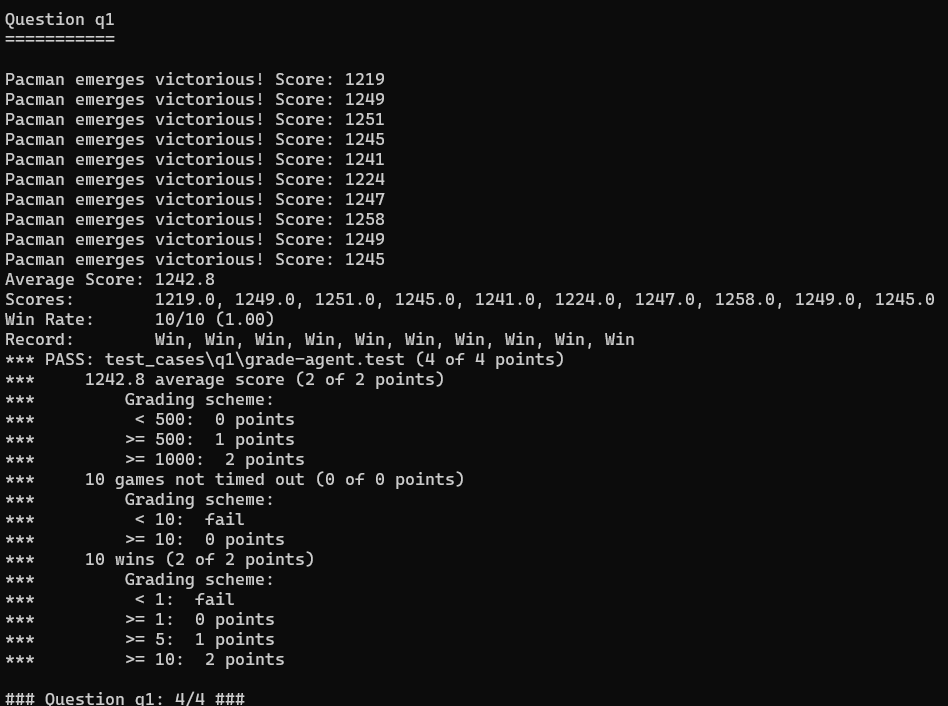
\includegraphics[width=12cm,height=9cm]{1.png}
    \end{figure}

    \normalsize{
        \hspace{1cm}在测试样例中,我们通过测试结果可以看出,测试程序
        在$openClassic$布局上运行我们给定的函数10次,根据我们程序运行结果
        的好坏给出评分。\\
    }
    \newpage
    \large{
        \hspace{1cm}\textbf{
            Question 2 (5 points): Minimax\\
        }
    }
    \begin{figure}[h]
        \centering
        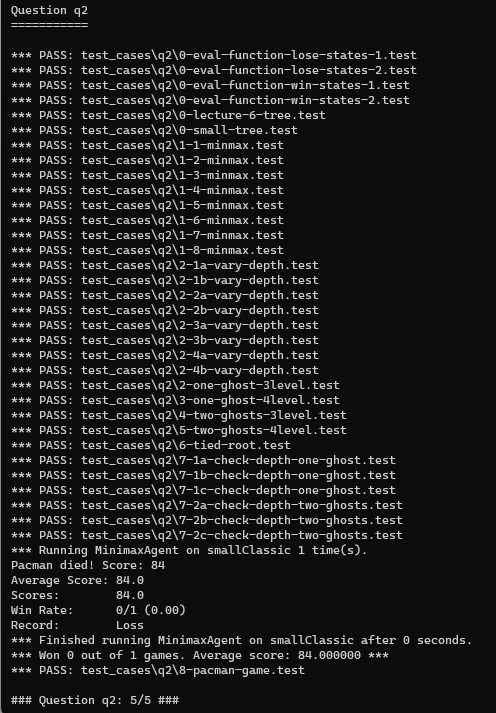
\includegraphics[width=12cm,height=16cm]{2.png}
    \end{figure}
    \normalsize{
        \hspace{1cm}在$Minmax()$测试中,测试程序将会确定我们编写的$Minmax()$算法中
        是否探索了正确数量的游戏状态,这是$Minmax()$检测中唯一可靠的方法,因此$autograder$
        会非常挑剔我们函数的调用次数最后给出评分。\\
    }
    \newpage
    \large{
        \hspace{1cm}\textbf{
            Question 3 (5 points): Alpha-Beta Pruning\\
        }
    }
    \begin{figure}[h]
        \centering
        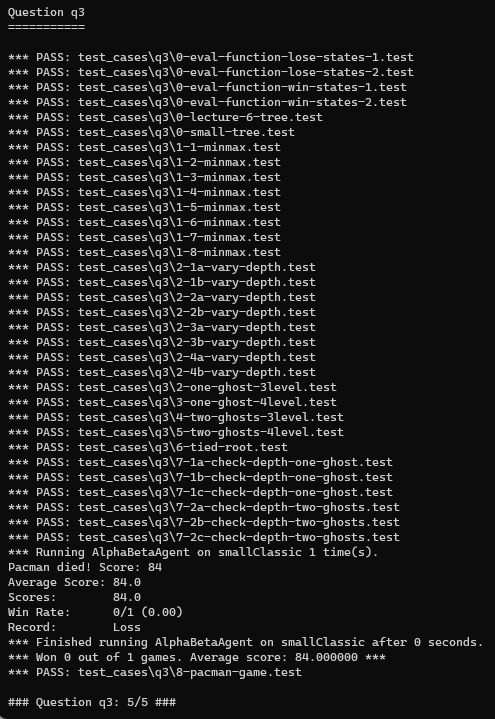
\includegraphics[width=12cm,height=16cm]{3.png}
    \end{figure}
    \normalsize{
        \hspace{1cm}在测试$Alpha-Beta$算法时,测试程序会检查我们的代码是否探索了
        正确数量的状态,所以我们执行$alpha-beta$修剪而不重新排序子项很重要。\\
    }
    \newpage
    \large{
        \hspace{1cm}\textbf{
            Question 4 (5 points): Expectimax\\
        }
    }
    \begin{figure}[h]
        \centering
        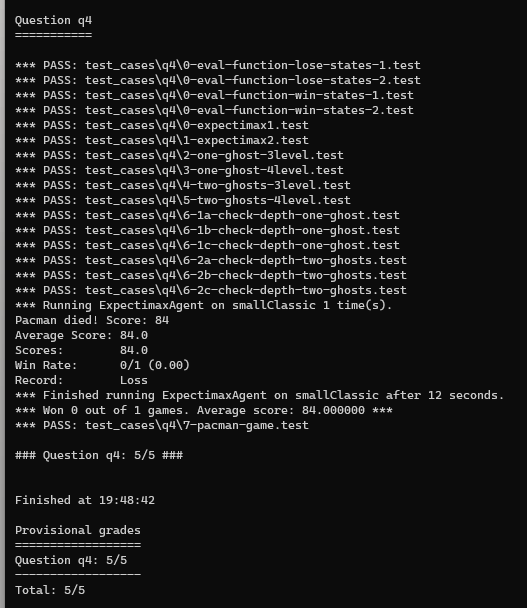
\includegraphics[width=12cm,height=12cm]{4.png}
    \end{figure}
    \normalsize{
        \hspace{1cm}第四个子任务是针对更一般的情况下的检查,要求我们在$Minmax()$基础上进行细节的改进。\\
    }
    \newpage
    \large{
        \hspace{1cm}\textbf{
            Question 5 (6 points): Evaluation Function\\
        }
    }
    \begin{figure}[h]
        \centering
        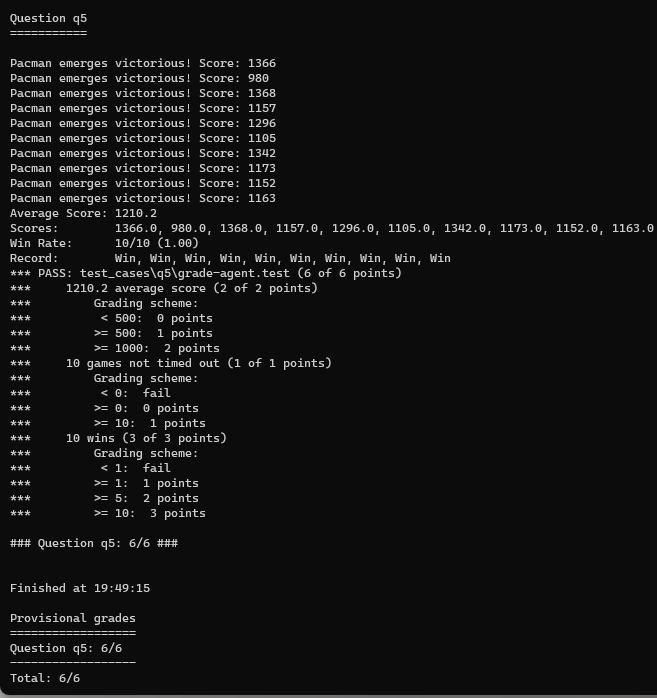
\includegraphics[width=12cm,height=12cm]{5.png}
    \end{figure}
    \normalsize{
        \hspace{1cm}在本测试用例中,测试程序将在$smallClassic$布局上运行十次我们
        的函数并根据具体函数得到结果的好坏进行评分。\\
    }
    \large{
        \hspace{1cm}\textbf{
           总测试结果如下:\\
        }
    }
    \begin{figure}[h]
        \centering
        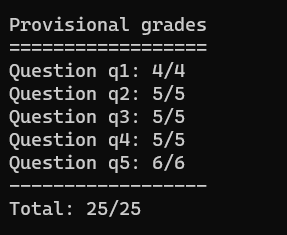
\includegraphics[width=12cm,height=6cm]{all.png}
    \end{figure}
    \newpage
    \Large{
        \textbf{
            五、总结与分析\\
        }
    }
    \large{
        \textbf{
            1、完成项目中遇到的问题\\
        }
    }
    \normalsize{
       \hspace{1cm}(1)在完成本次项目$project2$时,相比$project1$,我对这类的大型项目上手更快,阅读代码并理解其基础用法也变得更快,
       本次项目主要考察博弈对抗搜索,有新颖的知识点,也有教材上经典的算法复现(如$\alpha \beta$剪枝等),我遇到的第一个问题是子任务1,在要求设计
       评估函数时,我一时不知该从何下手,多次尝试但结果总不是最优,于是我认真分析该问题本质,从"趋利避害"的基本原则出发,在反复调节参数的情况下解决了
       问题。\\
       \hspace{1cm}(2)第二个主要的问题是$Minmax()$算法的编写,本项目涉及的是一对多的对抗搜索,所以$MinValue()$不能完全模仿书上的算法模板完成,
       每次的$ghost layer$我们需要枚举所有的$ghost$的可能状态之后才能进入$MaxValue()$函数,本来我考虑通过循环枚举实现,但由于ghost的数量以及其
       可能的后续状态都不确定,实现起来太过复杂,最后采用了递归方式才得以解决。\\
    }
    \large{
        \textbf{
            2、本项目中的收获与思考\\
        }
    }
    \normalsize{
        \hspace{1cm}通过该项目的完成,首先我对$python$中的许多基本用法相比之前又有了更深的了解,对于这种大型$python$类搭建构成的
        大型项目也有了更深刻的理解,其次就是有关算法的收获,在本次项目中我自己完成了$python$语言编写的$Minmax$算法,$\alpha \beta$剪枝,对于这类人工智能领域中
        的对抗搜索问题有了更深的认识于理解。\\
    }
}
\end{flushleft}
\end{document}

